\vspace{-10pt}
%\section{Automatic I/O Activity Management Using Program Contexts}
\section{\note{Automatic I/O Activity Management}}
\label{sec:programcontext}
\vspace{-5pt}
\begin{figure}[t]
%	\vspace{-10pt}
	\centering
	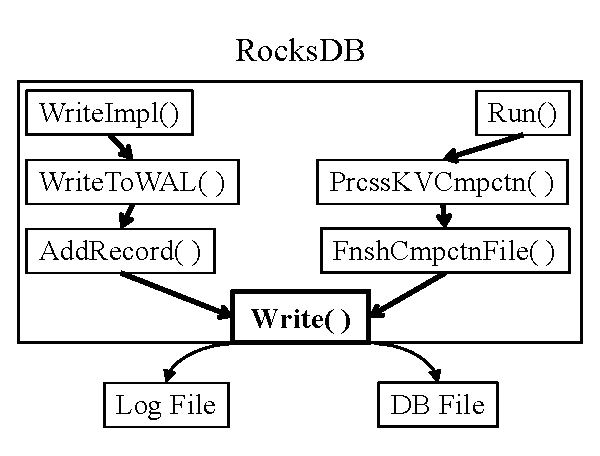
\includegraphics[width=0.4\textwidth]{figure/writepath}
	\vspace{-5pt}
	\caption{An illustration of (simplified) execution paths of two dominant I/O activities in RocksDB.}
	\label{fig:iopath}
	\vspace{-10pt}
\end{figure}

In developing an efficient data lifetime separator for general I/O workloads,
our key insight was that in most applications, the overall I/O behavior of
applications is decided by a few dominant I/O activities ({\it e.g.}, logging and
flushing in RocksDB).  Moreover, data written by dominant I/O activities tend
to have distinct lifetime patterns.  Therefore, if such dominant I/O activities
of applications can be automatically detected and distinguished each other in
an LBA-{\it oblivious} fashion, an automatic stream management technique can be
developed for widely varying I/O workloads including append-only workloads.

In this paper, we argue that a program context can be used to build an
efficient general-purpose classifier of dominant I/O activities with different
data lifetimes.  Here, a PC represents an execution path of an application
which invokes write-related system call functions such as {\tt write()} and
{\tt writev()}.  There could be various ways of extracting PCs, but the most
common approach~\cite{PC, PC2} is to represent each PC with its PC signature
which is computed by summing program counter values of all the functions along
the execution path which leads to a write system call.

%we represent the PC by summing program counter values of
%all the functions along the execution path which leads to a write system call.

\begin{figure*}[!t]
\centering
%\vspace{-10pt}
	\subfloat[RocksDB: Logging]{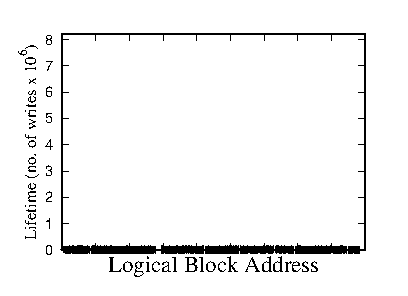
\includegraphics[width=0.22\textwidth]{figure/pcID_2_new.eps}} % data from 4/03031953 
	\hspace{10pt}
	\subfloat[RocksDB: Flushing]{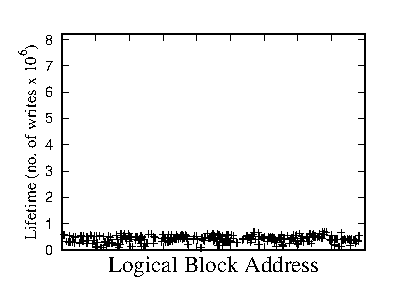
\includegraphics[width=0.22\textwidth]{figure/pcID_3_new.eps}}
	\hspace{10pt}
	\subfloat[RocksDB: Compaction]{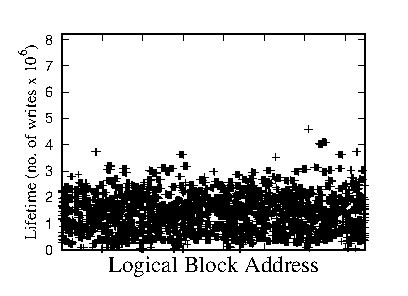
\includegraphics[width=0.22\textwidth]{figure/pc_3_new.eps}}  % data from 4/03040047

	\hfill

	\vspace{-10pt}
	\subfloat[SQLite: Logging]{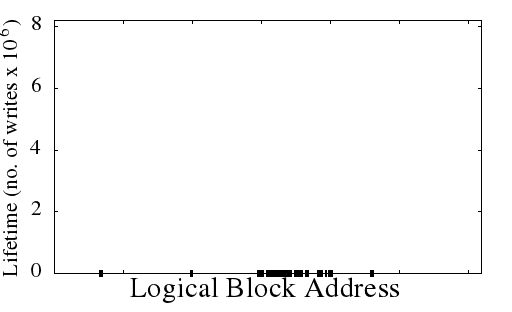
\includegraphics[width=0.22\textwidth]{figure/sqlite_pcID_3_new.eps}}
	\hspace{2pt}
	\subfloat[SQLite: Updating]{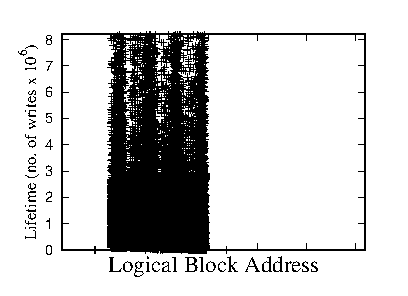
\includegraphics[width=0.22\textwidth]{figure/sqlite_pcID_1_new.eps}}
	\hspace{2pt}
	\subfloat[GCC: Outputting Temp]{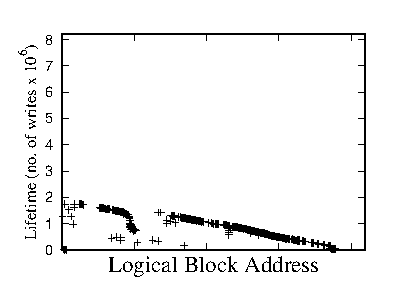
\includegraphics[width=0.22\textwidth]{figure/gcc_pcID_1_new.eps}}
	\hspace{2pt}
	\subfloat[GCC: Outputting Executable]{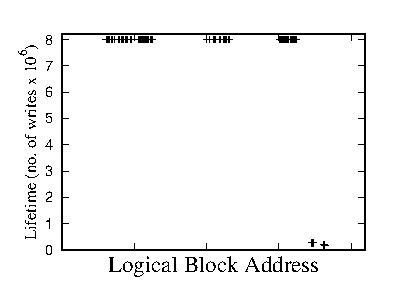
\includegraphics[width=0.22\textwidth]{figure/gcc_pcID_8_new.eps}}
\vspace{-5pt}
\caption{Data lifetime distributions of dominant I/O activities in RocksDB, SQLite and GCC.} 
\label{fig:types_and_PCs}
\vspace{-10pt}
\end{figure*}

\vspace{-10pt}
%\subsection{Program Context as a Unit of Lifetime Classification}
\subsection{\note{PC as a Unit of Lifetime Classification}}
\vspace{-5pt}
In order to illustrate that using PCs is an effective way to distinguish I/O
activities of an application and their data lifetime patterns, we measured data
lifetime distributions of PCs from various applications with different I/O
workloads.  In this section, we report our evaluation results for three
applications with distinct I/O activities: RocksDB~\cite{RocksDB},
SQLite~\cite{SQLite}, and GCC~\cite{GCC}.  RocksDB shows the append-only
workload while SQLite shows a workload that updates in place.  Both database
workloads are expected to have distinct I/O activities for writing log files
and data files.  GCC represents an extensive compiler workload ({\it e.g.},
compiling a Linux kernel) that generates many short-lived temporary files ({\it
e.g.}, \texttt{.s}, \texttt{.d}, and \texttt{.rc} files) as well as some
long-lived files ({\it e.g.}, object files and kernel image files).

In RocksDB, dominant I/O activities include logging, flushing and compaction.
Since these I/O activities are invoked through different function-call paths,
we can easily identify dominant I/O activities of RocksDB using PCs.  For
example, Fig.~\ref{fig:iopath} shows (simplified) execution paths for logging
and compaction in RocksDB.  The sum of program counter values of the execution
path \texttt{WriteImpl()}$\rightarrow$\texttt{WriteToWAL()}$\rightarrow$
\texttt{AddRecord()} is used to represent a PC for the logging activity while
that of the execution path \texttt{Run()}$\rightarrow$
\texttt{ProcessKeyValueCompaction()} $\rightarrow$
\texttt{FinishCompactionFile()} is used for the compaction activity.
In SQLite, there exist two dominant I/O activities which are logging and
managing database tables.  Similar to the RocksDB, SQLite writes log files and
database files using different execution paths.  In GCC, there exist many
dominant I/O activities of creating various types of temporal files and object
files.

%\textcolor{red}{(TODO: 갑자기
%lifetime 이야기가 나옴. 없애도 큰 문제가 없을 듯...) \sout{Note that using a
%program context to distinguish data lifetimes is not new. For example, Ha {\it
%et al.} proposed a data separation technique based on the program
%context~\cite{PCHa}.  However, their work was neither designed for append-only
%workloads nor for modern multi-streamed SSDs.}}

To confirm our hypothesis that data lifetimes can be distinguished by tracking
dominant I/O activities and a PC is a useful unit of classification for
different I/O activities, we have analyzed how well PCs work for RocksDB,
SQLite and GCC.  Fig.~\ref{fig:types_and_PCs} shows data lifetime distributions
of dominant I/O activities which were distinguished by computed PC values.  As
expected, Fig.~\ref{fig:types_and_PCs} validates that dominant I/O activities
show distinct data lifetime distributions over the logical address space.  For
example, as shown in
Figs.~\ref{fig:types_and_PCs}(a)$\sim$\ref{fig:types_and_PCs}(c), the logging
activity, the flushing activity and the compaction activity in RocksDB clearly
exhibit quite different data lifetime distributions.  While the logged data
written by the logging activity have short lifetimes, the flushed data by the
flushing activity have little bit longer lifetimes.  Similarly, for SQLite and
GCC, dominant I/O activities show quite distinct data lifetime characteristics
as shown in Figs.~\ref{fig:types_and_PCs}(d)$\sim$\ref{fig:types_and_PCs}(e).
As shown in Figs.~\ref{fig:types_and_PCs}(d), the logging activity of SQLite
generates short-lived data.  This is because SQLite overwrites logging data in
a small and fixed storage space and then removes them soon.  Lifetimes of
temporary files generated by GCC are relatively short as shown in
Fig.~\ref{fig:types_and_PCs}(f), because of the write-once pattern of temporary
files.  But, unlike the other graphs in Fig.~\ref{fig:types_and_PCs}, data
lifetime distributions of Figs.~\ref{fig:types_and_PCs}(c) and
\ref{fig:types_and_PCs}(e), which correspond to the compaction activity of
RocksDB and the updating activity of SQLite, respectively, show large
variances.  These {\it outlier I/O activities} need a special treatment, which
will be described in Section 4.

Note that if we used an LBA-based data separator instead of the proposed
PC-based scheme, most of data lifetime characteristics shown in
Fig.~\ref{fig:types_and_PCs} could not have been known.  Only the data lifetime
distribution of the logging activity of SQLite, as shown in
Fig.~\ref{fig:types_and_PCs}(d), can be accurately captured by the LBA-based
data separator.  For example, the LBA-based data separtor cannot decide that
the data lifetime of data produced from the outputting temp activity of GCC is
short because temporary files are not written at the same LBA each time they
are generated during the compiling step. 


\vspace{-10pt}
\subsection{Extracting PCs}
\vspace{-5pt}
As mentioned earlier, a PC signature, which is used as a unique ID of each
program context, is defined to be the sum of program counters along the
execution path of function calls that finally reaches a write-related system
function.  In theory, program counter values in the execution path can be
extracted in a relatively straightforward manner.  Except for inline functions,
every function call involves pushing the address of the next instruction of a
caller as a return address to the stack, followed by pushing a frame pointer
value.  By referring to frame pointers, we can back-track stack frames of a
process and selectively get return addresses for generating a PC signature.
Fig.~\ref{fig:getpc}(a) illustrates a stack of RocksDB corresponding to
Fig.~\ref{fig:iopath}, where return addresses are pushed before calling
\texttt{write()}, \texttt{AddRecord()} and \texttt{WriteToWAL()}.  Since frame
pointer values in the stack hold the addresses of previous frame pointers, we
can obtain return addresses and accumulate them to compute a PC signature.  

%For example,
%Fig.~\ref{fig:getpc}(a) shows abstracted execution paths of log data and
%compaction data in RocksDB.  The return addresses are pushed before calling the
%\textsf{\small  write()}, \textsf{\small AddRecord()} and \textsf{\small
%WriteToWAL()} functions.  Fig.~\ref{fig:getpc}(b) illustrates how a PC
%signature is obtained by back-tracking the stack.  Since frame pointer values
%in the stack hold the addresses of previous frame pointers, we can easily
%obtain return addresses and accumulate them to compute a PC signature.  

The frame pointer-based approach for computing a PC signature, however, is not
always possible because modern C/C++ compilers often do not use a frame pointer
for improving the efficiency of register allocation.  One example is a {\tt
-fomit-frame-pointer} option of GCC~\cite{GCC}.  This option enables to use a frame
pointer as a general-purpose register for performance, but makes it difficult for us
to back-track return addresses along the call chains.  

\begin{figure}[t]
%	\vspace{-10pt}
	\centering
	%\vspace{-8pt}
	%\subfloat[Abstracted execution paths of two I/O activities of RocksDB.]{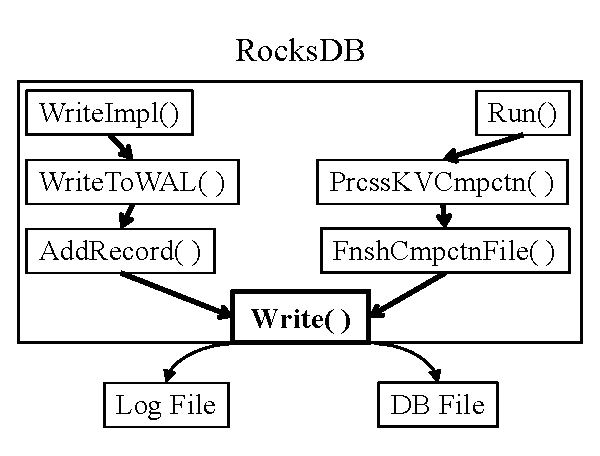
\includegraphics[width=0.3\textwidth]{figure/writepath}}  
	%\vspace{-14pt}
	%\hfill
	\subfloat[with the frame pointer.]{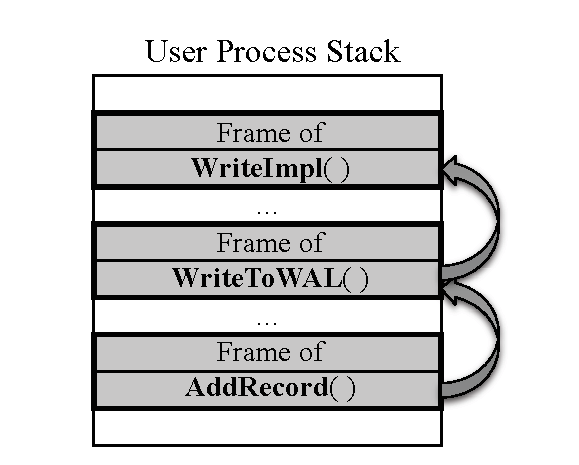
\includegraphics[width=0.23\textwidth]{figure/getpc_new1}}
	%\hspace{10pt}
	\subfloat[without the frame pointer.]{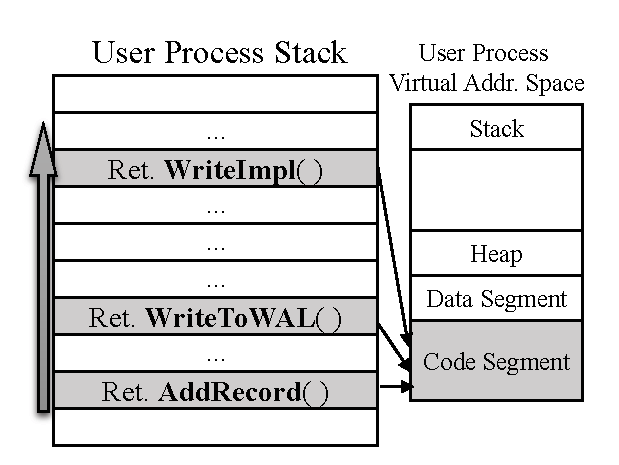
\includegraphics[width=0.248\textwidth]{figure/getpc2}}
	%\vspace{-9pt}
	\caption{Examples of PC extraction methods.}
	%\caption{An example execution path and its PC extraction.} %shane part
	\label{fig:getpc}
	\vspace{-10pt}
\end{figure}

We employ a simple but effective workaround for back-tracking a call stack when
a frame pointer is not available.  When a write system call is made,
we scan every word in the stack
and checks if it belongs to process's code segment.  If the scanned stack word
holds a value within the address range of the code segment, it assumes that it
is a return address.  Since scanning the entire stack may takes too long, we stop
the scanning step once a sufficient number of return address candidates are found.
In the current implementation, the scanning process stops early once 
five return address candidates are identified.  
Even though it is quite ad-hoc, this restricted scan is quite effective
in distinguishing different PCs because it is very unlikely that two different PCs
reach the same \texttt{write()} system call through the same execution subpath 
that covers five proceeding function calls. 
In our evaluation on a PC with 3.4 GHz Intel CPU, the overhead of the
restricted scan was almost negligible, taking only 300$\sim$400 $n$sec per
\texttt{write()} system call.

